% !TEX program = xelatex
\documentclass[UTF8,fontset=fandol,a4paper,11pt]{ctexart}
\usepackage[margin=21mm,top=23mm,bottom=22mm,headheight=16pt]{geometry}
\usepackage{amsmath,amssymb,mathtools,bm}
\usepackage{tikz}
\usetikzlibrary{arrows.meta,calc,angles,quotes,patterns}
\usepackage{xcolor,booktabs,array,longtable,enumitem,fancyhdr,needspace}
\usepackage[unicode,hidelinks]{hyperref}
\definecolor{ink}{HTML}{24343C}
\definecolor{accent}{HTML}{166A70}
\definecolor{muted}{HTML}{65747A}
\definecolor{rulegray}{HTML}{D4DDE0}
\definecolor{warm}{HTML}{966037}
\color{ink}
\setlength{\parindent}{2em}
\setlength{\parskip}{4pt}
\linespread{1.12}
\AtBeginDocument{\setlength{\abovedisplayskip}{6pt plus 2pt minus 1pt}
\setlength{\belowdisplayskip}{6pt plus 2pt minus 1pt}
\setlength{\abovedisplayshortskip}{0pt plus 1pt}
\setlength{\belowdisplayshortskip}{4pt plus 1pt}}
\setlist[enumerate]{label=(\arabic*),leftmargin=2.3em,itemsep=3pt,topsep=4pt}
\setlist[itemize]{leftmargin=2em,itemsep=2pt,topsep=4pt}
\allowdisplaybreaks[1]
\setlength{\emergencystretch}{2em}
\setcounter{secnumdepth}{0}
\providecommand{\tightlist}{\setlength{\itemsep}{0pt}\setlength{\parskip}{0pt}}
\ctexset{section={format=\Large\bfseries\color{accent},beforeskip=10pt,afterskip=9pt},
subsection={format=\normalsize\bfseries\color{accent},beforeskip=10pt,afterskip=4pt},
subsubsection={format=\normalsize\bfseries,beforeskip=8pt,afterskip=3pt}}
\pagestyle{fancy}
\fancyhf{}
\fancyhead[L]{\small\color{muted}物理学难题集萃}
% 页眉仅保留书名；版本名称只在封面显示。
\fancyfoot[L]{\small\color{muted}\chapterlabel}
\fancyfoot[R]{\small\thepage}
\renewcommand{\headrulewidth}{0.4pt}
\renewcommand{\footrulewidth}{0pt}
\newcommand{\dd}{\mathop{}\!\mathrm{d}}
\newcommand{\vect}[1]{\bm{#1}}
\newcommand{\tagline}[1]{\noindent{\small\color{muted}#1}\par}
\newcommand{\result}[1]{\begin{equation*}\boxed{#1}\end{equation*}}
\newcommand{\figcaption}[1]{\par\vspace{2pt}{\small\color{muted}#1}\par}
\newcommand{\teach}[2]{\Needspace{4\baselineskip}\subsection*{讲解要点与追问}#1\par\smallskip\noindent\textbf{追问：}#2\par}
\newcommand{\workarea}{\par\vspace{7mm}\noindent{\small\color{muted}作答区}\par\vspace{4mm}
\noindent\textcolor{rulegray}{\rule{\linewidth}{0.3pt}}\par\vspace{16mm}
\noindent\textcolor{rulegray}{\rule{\linewidth}{0.3pt}}\par\vspace{16mm}
\noindent\textcolor{rulegray}{\rule{\linewidth}{0.3pt}}\par\vspace{16mm}
\noindent\textcolor{rulegray}{\rule{\linewidth}{0.3pt}}}
\tikzset{axis/.style={-{Stealth[length=2mm]},thin,color=muted},
motion/.style={-{Stealth[length=2.3mm]},thick,color=accent},
force/.style={-{Stealth[length=2.3mm]},thick,color=warm},
traj/.style={thick,color=accent},guide/.style={dashed,thin,color=muted},
object/.style={thick,color=ink},every node/.style={font=\small}}\widowpenalty=10000\clubpenalty=10000\displaywidowpenalty=10000\newcommand{\chapterlabel}{光学第五章\quad 光的色散、散射和吸收}







\hypersetup{pdftitle={光学第五章 光的色散、散射和吸收·学生版},pdfauthor={}}

\begin{document}\pdfbookmark[0]{光学第五章 光的色散、散射和吸收}{cover}

\thispagestyle{empty}\vspace*{22mm}

\noindent{\Huge\bfseries 物理学难题集萃}\par\vspace{10mm}

\noindent{\LARGE 光学第五章}\par\vspace{6mm}

\noindent{\LARGE 光的色散、散射和吸收}\par\vspace{12mm}

\noindent{\Large\color{accent}学生版}\par\vspace{9mm}

\noindent\textcolor{accent}{\rule{\linewidth}{1pt}}\par\vspace{9mm}

\noindent 第1--11题\par\vfill\clearpage

\pdfbookmark[1]{题目目录}{contents}\section*{题目目录}

\begin{longtable}{@{}r p{113mm} r@{}}\toprule 题号 & 题目 & 页码\\\midrule

\hyperref[q:1]{1} & \hyperref[q:1]{玻璃中的相速与群速} & \pageref{q:1} \\

\hyperref[q:2]{2} & \hyperref[q:2]{氢气的有效共振与振子参数} & \pageref{q:2} \\

\hyperref[q:3]{3} & \hyperref[q:3]{双共振色散与质量比} & \pageref{q:3} \\

\hyperref[q:4]{4} & \hyperref[q:4]{X射线色散及速度乘积} & \pageref{q:4} \\

\hyperref[q:5]{5} & \hyperref[q:5]{金属自由电子响应与反射} & \pageref{q:5} \\

\hyperref[q:6]{6} & \hyperref[q:6]{电离层的反射与布儒斯特角} & \pageref{q:6} \\

\hyperref[q:7]{7} & \hyperref[q:7]{麦克斯韦方程的纵向模式} & \pageref{q:7} \\

\hyperref[q:8]{8} & \hyperref[q:8]{均匀介质与涨落散射} & \pageref{q:8} \\

\hyperref[q:9]{9} & \hyperref[q:9]{密度涨落的瑞利散射} & \pageref{q:9} \\

\hyperref[q:10]{10} & \hyperref[q:10]{射电脉冲啁啾与电子密度} & \pageref{q:10} \\

\hyperref[q:11]{11} & \hyperref[q:11]{吸收系数测量与表面反射} & \pageref{q:11} \\

\bottomrule\end{longtable}

\clearpage

\pdfbookmark[2]{第 1 题 玻璃中的相速与群速}{q1}

\section*{第 1 题\quad 玻璃中的相速与群速}\label{q:1}

冕牌玻璃K9的色散用柯西公式描述：
\[
n(\lambda_0)=A+\frac B{\lambda_0^2}+\frac C{\lambda_0^4},
\quad A=1.504,\quad B=4.437\times10^3\,\mathrm{nm^2},\quad C=-1.387\times10^8\,\mathrm{nm^4}.
\]
钠黄双线的平均真空波长为$589.3\,\mathrm{nm}$，另给该处折射率$n_D=1.51630$。求相速、群速，比较两者；检查两组折射率数据是否完全一致，并说明所用近似。取$c=3.00\times10^8\,\mathrm{m/s}$。

\begin{center}\begin{minipage}{.98\linewidth}\centering
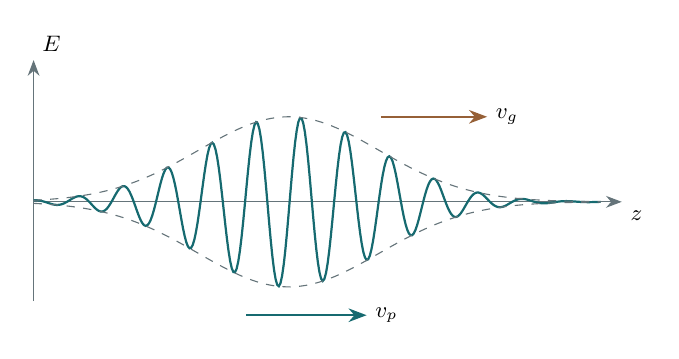
\begin{tikzpicture}[scale=.9,transform shape]
\draw[axis] (0.00000,0.00000)--(8.30000,0.00000);\draw[axis] (0.00000,-1.40000)--(0.00000,2.00000);\node[below right] at (8.30000,0.00000) {$z$};\node[above right] at (0.00000,2.00000) {$E$};\draw[traj] plot coordinates {(0.00000,0.02198) (0.02292,0.02252) (0.04585,0.02181) (0.06877,0.01976) (0.09169,0.01635) (0.11461,0.01164) (0.13754,0.00576) (0.16046,-0.00105) (0.18338,-0.00850) (0.20630,-0.01621) (0.22923,-0.02377) (0.25215,-0.03072) (0.27507,-0.03658) (0.29799,-0.04093) (0.32092,-0.04334) (0.34384,-0.04351) (0.36676,-0.04120) (0.38968,-0.03630) (0.41261,-0.02886) (0.43553,-0.01907) (0.45845,-0.00728) (0.48138,0.00603) (0.50430,0.02023) (0.52722,0.03457) (0.55014,0.04824) (0.57307,0.06041) (0.59599,0.07022) (0.61891,0.07692) (0.64183,0.07984) (0.66476,0.07849) (0.68768,0.07258) (0.71060,0.06205) (0.73352,0.04711) (0.75645,0.02824) (0.77937,0.00620) (0.80229,-0.01802) (0.82521,-0.04322) (0.84814,-0.06804) (0.87106,-0.09105) (0.89398,-0.11078) (0.91691,-0.12585) (0.93983,-0.13505) (0.96275,-0.13738) (0.98567,-0.13219) (1.00860,-0.11920) (1.03152,-0.09854) (1.05444,-0.07081) (1.07736,-0.03705) (1.10029,0.00127) (1.12321,0.04234) (1.14613,0.08402) (1.16905,0.12402) (1.19198,0.15996) (1.21490,0.18953) (1.23782,0.21063) (1.26074,0.22147) (1.28367,0.22077) (1.30659,0.20776) (1.32951,0.18236) (1.35244,0.14516) (1.37536,0.09749) (1.39828,0.04132) (1.42120,-0.02074) (1.44413,-0.08560) (1.46705,-0.14982) (1.48997,-0.20976) (1.51289,-0.26183) (1.53582,-0.30264) (1.55874,-0.32923) (1.58166,-0.33929) (1.60458,-0.33128) (1.62751,-0.30460) (1.65043,-0.25965) (1.67335,-0.19791) (1.69628,-0.12185) (1.71920,-0.03491) (1.74212,0.05871) (1.76504,0.15416) (1.78797,0.24626) (1.81089,0.32975) (1.83381,0.39956) (1.85673,0.45113) (1.87966,0.48069) (1.90258,0.48551) (1.92550,0.46410) (1.94842,0.41638) (1.97135,0.34371) (1.99427,0.24891) (2.01719,0.13618) (2.04011,0.01088) (2.06304,-0.12067) (2.08596,-0.25152) (2.10888,-0.37445) (2.13181,-0.48238) (2.15473,-0.56876) (2.17765,-0.62795) (2.20057,-0.65558) (2.22350,-0.64888) (2.24642,-0.60684) (2.26934,-0.53037) (2.29226,-0.42234) (2.31519,-0.28744) (2.33811,-0.13204) (2.36103,0.03613) (2.38395,0.20835) (2.40688,0.37538) (2.42980,0.52794) (2.45272,0.65725) (2.47564,0.75549) (2.49857,0.81631) (2.52149,0.83522) (2.54441,0.80988) (2.56734,0.74032) (2.59026,0.62901) (2.61318,0.48075) (2.63610,0.30254) (2.65903,0.10321) (2.68195,-0.10703) (2.70487,-0.31707) (2.72779,-0.51555) (2.75072,-0.69145) (2.77364,-0.83468) (2.79656,-0.93675) (2.81948,-0.99117) (2.84241,-0.99394) (2.86533,-0.94378) (2.88825,-0.84228) (2.91117,-0.69384) (2.93410,-0.50554) (2.95702,-0.28675) (2.97994,-0.04869) (3.00287,0.19617) (3.02579,0.43478) (3.04871,0.65420) (3.07163,0.84233) (3.09456,0.98858) (3.11748,1.08448) (3.14040,1.12418) (3.16332,1.10480) (3.18625,1.02663) (3.20917,0.89316) (3.23209,0.71090) (3.25501,0.48911) (3.27794,0.23926) (3.30086,-0.02553) (3.32378,-0.29122) (3.34670,-0.54361) (3.36963,-0.76909) (3.39255,-0.95543) (3.41547,-1.09242) (3.43840,-1.17248) (3.46132,-1.19105) (3.48424,-1.14688) (3.50716,-1.04210) (3.53009,-0.88212) (3.55301,-0.67536) (3.57593,-0.43275) (3.59885,-0.16719) (3.62178,0.10718) (3.64470,0.37574) (3.66762,0.62420) (3.69054,0.83936) (3.71347,1.00984) (3.73639,1.12672) (3.75931,1.18396) (3.78223,1.17875) (3.80516,1.11169) (3.82808,0.98667) (3.85100,0.81068) (3.87393,0.59341) (3.89685,0.34670) (3.91977,0.08388) (3.94269,-0.18098) (3.96562,-0.43379) (3.98854,-0.66128) (4.01146,-0.85165) (4.03438,-0.99522) (4.05731,-1.08494) (4.08023,-1.11673) (4.10315,-1.08966) (4.12607,-1.00598) (4.14900,-0.87093) (4.17192,-0.69242) (4.19484,-0.48059) (4.21777,-0.24717) (4.24069,-0.00489) (4.26361,0.23330) (4.28653,0.45487) (4.30946,0.64842) (4.33238,0.80428) (4.35530,0.91496) (4.37822,0.97555) (4.40115,0.98393) (4.42407,0.94079) (4.44699,0.84958) (4.46991,0.71623) (4.49284,0.54877) (4.51576,0.35689) (4.53868,0.15132) (4.56160,-0.05675) (4.58453,-0.25628) (4.60745,-0.43697) (4.63037,-0.58982) (4.65330,-0.70757) (4.67622,-0.78501) (4.69914,-0.81926) (4.72206,-0.80981) (4.74499,-0.75851) (4.76791,-0.66937) (4.79083,-0.54829) (4.81375,-0.40270) (4.83668,-0.24107) (4.85960,-0.07246) (4.88252,0.09401) (4.90544,0.24966) (4.92837,0.38668) (4.95129,0.49854) (4.97421,0.58028) (4.99713,0.62874) (5.02006,0.64263) (5.04298,0.62257) (5.06590,0.57096) (5.08883,0.49177) (5.11175,0.39029) (5.13467,0.27278) (5.15759,0.14609) (5.18052,0.01727) (5.20344,-0.10681) (5.22636,-0.21984) (5.24928,-0.31636) (5.27221,-0.39205) (5.29513,-0.44387) (5.31805,-0.47021) (5.34097,-0.47087) (5.36390,-0.44704) (5.38682,-0.40116) (5.40974,-0.33670) (5.43266,-0.25797) (5.45559,-0.16982) (5.47851,-0.07736) (5.50143,0.01433) (5.52436,0.10047) (5.54728,0.17683) (5.57020,0.23991) (5.59312,0.28711) (5.61605,0.31681) (5.63897,0.32840) (5.66189,0.32229) (5.68481,0.29978) (5.70774,0.26299) (5.73066,0.21467) (5.75358,0.15802) (5.77650,0.09651) (5.79943,0.03367) (5.82235,-0.02714) (5.84527,-0.08282) (5.86819,-0.13078) (5.89112,-0.16896) (5.91404,-0.19596) (5.93696,-0.21106) (5.95989,-0.21423) (5.98281,-0.20606) (6.00573,-0.18770) (6.02865,-0.16080) (6.05158,-0.12732) (6.07450,-0.08947) (6.09742,-0.04952) (6.12034,-0.00973) (6.14327,0.02783) (6.16619,0.06134) (6.18911,0.08931) (6.21203,0.11065) (6.23496,0.12472) (6.25788,0.13128) (6.28080,0.13054) (6.30372,0.12305) (6.32665,0.10971) (6.34957,0.09165) (6.37249,0.07017) (6.39542,0.04665) (6.41834,0.02249) (6.44126,-0.00099) (6.46418,-0.02260) (6.48711,-0.04135) (6.51003,-0.05648) (6.53295,-0.06746) (6.55587,-0.07406) (6.57880,-0.07626) (6.60172,-0.07430) (6.62464,-0.06863) (6.64756,-0.05984) (6.67049,-0.04866) (6.69341,-0.03586) (6.71633,-0.02227) (6.73926,-0.00866) (6.76218,0.00425) (6.78510,0.01582) (6.80802,0.02558) (6.83095,0.03315) (6.85387,0.03832) (6.87679,0.04104) (6.89971,0.04137) (6.92264,0.03951) (6.94556,0.03574) (6.96848,0.03045) (6.99140,0.02404) (7.01433,0.01696) (7.03725,0.00965) (7.06017,0.00250) (7.08309,-0.00410) (7.10602,-0.00988) (7.12894,-0.01459) (7.15186,-0.01808) (7.17479,-0.02030) (7.19771,-0.02123) (7.22063,-0.02096) (7.24355,-0.01962) (7.26648,-0.01738) (7.28940,-0.01445) (7.31232,-0.01104) (7.33524,-0.00740) (7.35817,-0.00373) (7.38109,-0.00024) (7.40401,0.00291) (7.42693,0.00559) (7.44986,0.00769) (7.47278,0.00918) (7.49570,0.01003) (7.51862,0.01026) (7.54155,0.00992) (7.56447,0.00910) (7.58739,0.00789) (7.61032,0.00639) (7.63324,0.00471) (7.65616,0.00296) (7.67908,0.00125) (7.70201,-0.00034) (7.72493,-0.00174) (7.74785,-0.00289) (7.77077,-0.00376) (7.79370,-0.00434) (7.81662,-0.00462) (7.83954,-0.00463) (7.86246,-0.00439) (7.88539,-0.00394) (7.90831,-0.00334) (7.93123,-0.00263) (7.95415,-0.00186) (7.97708,-0.00108) (8.00000,-0.00034)};\draw[guide] plot coordinates {(0.00000,0.02198) (0.02292,0.02312) (0.04585,0.02432) (0.06877,0.02557) (0.09169,0.02688) (0.11461,0.02824) (0.13754,0.02966) (0.16046,0.03115) (0.18338,0.03269) (0.20630,0.03431) (0.22923,0.03599) (0.25215,0.03774) (0.27507,0.03957) (0.29799,0.04147) (0.32092,0.04344) (0.34384,0.04550) (0.36676,0.04764) (0.38968,0.04986) (0.41261,0.05217) (0.43553,0.05456) (0.45845,0.05705) (0.48138,0.05964) (0.50430,0.06232) (0.52722,0.06510) (0.55014,0.06798) (0.57307,0.07097) (0.59599,0.07406) (0.61891,0.07726) (0.64183,0.08058) (0.66476,0.08401) (0.68768,0.08756) (0.71060,0.09123) (0.73352,0.09502) (0.75645,0.09893) (0.77937,0.10298) (0.80229,0.10716) (0.82521,0.11146) (0.84814,0.11591) (0.87106,0.12049) (0.89398,0.12522) (0.91691,0.13008) (0.93983,0.13509) (0.96275,0.14025) (0.98567,0.14556) (1.00860,0.15102) (1.03152,0.15664) (1.05444,0.16241) (1.07736,0.16834) (1.10029,0.17443) (1.12321,0.18068) (1.14613,0.18709) (1.16905,0.19367) (1.19198,0.20042) (1.21490,0.20733) (1.23782,0.21441) (1.26074,0.22166) (1.28367,0.22908) (1.30659,0.23668) (1.32951,0.24445) (1.35244,0.25239) (1.37536,0.26050) (1.39828,0.26879) (1.42120,0.27725) (1.44413,0.28588) (1.46705,0.29469) (1.48997,0.30367) (1.51289,0.31282) (1.53582,0.32214) (1.55874,0.33164) (1.58166,0.34130) (1.60458,0.35113) (1.62751,0.36113) (1.65043,0.37129) (1.67335,0.38161) (1.69628,0.39210) (1.71920,0.40274) (1.74212,0.41353) (1.76504,0.42448) (1.78797,0.43557) (1.81089,0.44681) (1.83381,0.45819) (1.85673,0.46971) (1.87966,0.48136) (1.90258,0.49315) (1.92550,0.50505) (1.94842,0.51708) (1.97135,0.52922) (1.99427,0.54147) (2.01719,0.55382) (2.04011,0.56627) (2.06304,0.57882) (2.08596,0.59145) (2.10888,0.60416) (2.13181,0.61694) (2.15473,0.62979) (2.17765,0.64269) (2.20057,0.65565) (2.22350,0.66866) (2.24642,0.68170) (2.26934,0.69477) (2.29226,0.70786) (2.31519,0.72096) (2.33811,0.73407) (2.36103,0.74717) (2.38395,0.76027) (2.40688,0.77333) (2.42980,0.78637) (2.45272,0.79937) (2.47564,0.81232) (2.49857,0.82522) (2.52149,0.83804) (2.54441,0.85079) (2.56734,0.86346) (2.59026,0.87602) (2.61318,0.88848) (2.63610,0.90083) (2.65903,0.91305) (2.68195,0.92514) (2.70487,0.93709) (2.72779,0.94888) (2.75072,0.96050) (2.77364,0.97196) (2.79656,0.98323) (2.81948,0.99431) (2.84241,1.00519) (2.86533,1.01586) (2.88825,1.02631) (2.91117,1.03653) (2.93410,1.04651) (2.95702,1.05625) (2.97994,1.06573) (3.00287,1.07494) (3.02579,1.08389) (3.04871,1.09256) (3.07163,1.10093) (3.09456,1.10901) (3.11748,1.11679) (3.14040,1.12426) (3.16332,1.13141) (3.18625,1.13824) (3.20917,1.14474) (3.23209,1.15090) (3.25501,1.15672) (3.27794,1.16219) (3.30086,1.16731) (3.32378,1.17207) (3.34670,1.17647) (3.36963,1.18050) (3.39255,1.18417) (3.41547,1.18745) (3.43840,1.19037) (3.46132,1.19290) (3.48424,1.19505) (3.50716,1.19681) (3.53009,1.19819) (3.55301,1.19918) (3.57593,1.19979) (3.59885,1.20000) (3.62178,1.19982) (3.64470,1.19926) (3.66762,1.19831) (3.69054,1.19697) (3.71347,1.19524) (3.73639,1.19313) (3.75931,1.19064) (3.78223,1.18776) (3.80516,1.18451) (3.82808,1.18089) (3.85100,1.17689) (3.87393,1.17253) (3.89685,1.16780) (3.91977,1.16272) (3.94269,1.15728) (3.96562,1.15150) (3.98854,1.14537) (4.01146,1.13891) (4.03438,1.13211) (4.05731,1.12499) (4.08023,1.11755) (4.10315,1.10981) (4.12607,1.10175) (4.14900,1.09341) (4.17192,1.08477) (4.19484,1.07585) (4.21777,1.06666) (4.24069,1.05721) (4.26361,1.04750) (4.28653,1.03754) (4.30946,1.02734) (4.33238,1.01691) (4.35530,1.00627) (4.37822,0.99541) (4.40115,0.98435) (4.42407,0.97309) (4.44699,0.96166) (4.46991,0.95005) (4.49284,0.93827) (4.51576,0.92634) (4.53868,0.91427) (4.56160,0.90206) (4.58453,0.88972) (4.60745,0.87727) (4.63037,0.86472) (4.65330,0.85206) (4.67622,0.83932) (4.69914,0.82650) (4.72206,0.81362) (4.74499,0.80067) (4.76791,0.78768) (4.79083,0.77464) (4.81375,0.76157) (4.83668,0.74848) (4.85960,0.73538) (4.88252,0.72227) (4.90544,0.70917) (4.92837,0.69608) (4.95129,0.68300) (4.97421,0.66996) (4.99713,0.65695) (5.02006,0.64399) (5.04298,0.63108) (5.06590,0.61822) (5.08883,0.60543) (5.11175,0.59271) (5.13467,0.58008) (5.15759,0.56752) (5.18052,0.55506) (5.20344,0.54270) (5.22636,0.53044) (5.24928,0.51829) (5.27221,0.50625) (5.29513,0.49433) (5.31805,0.48254) (5.34097,0.47087) (5.36390,0.45934) (5.38682,0.44794) (5.40974,0.43669) (5.43266,0.42558) (5.45559,0.41462) (5.47851,0.40381) (5.50143,0.39315) (5.52436,0.38265) (5.54728,0.37231) (5.57020,0.36214) (5.59312,0.35212) (5.61605,0.34228) (5.63897,0.33260) (5.66189,0.32309) (5.68481,0.31374) (5.70774,0.30458) (5.73066,0.29558) (5.75358,0.28675) (5.77650,0.27810) (5.79943,0.26962) (5.82235,0.26132) (5.84527,0.25319) (5.86819,0.24523) (5.89112,0.23745) (5.91404,0.22984) (5.93696,0.22240) (5.95989,0.21513) (5.98281,0.20803) (6.00573,0.20110) (6.02865,0.19434) (6.05158,0.18774) (6.07450,0.18131) (6.09742,0.17504) (6.12034,0.16894) (6.14327,0.16299) (6.16619,0.15721) (6.18911,0.15158) (6.21203,0.14610) (6.23496,0.14078) (6.25788,0.13560) (6.28080,0.13058) (6.30372,0.12570) (6.32665,0.12096) (6.34957,0.11636) (6.37249,0.11190) (6.39542,0.10758) (6.41834,0.10339) (6.44126,0.09933) (6.46418,0.09540) (6.48711,0.09160) (6.51003,0.08792) (6.53295,0.08436) (6.55587,0.08092) (6.57880,0.07759) (6.60172,0.07437) (6.62464,0.07127) (6.64756,0.06827) (6.67049,0.06538) (6.69341,0.06259) (6.71633,0.05990) (6.73926,0.05731) (6.76218,0.05481) (6.78510,0.05240) (6.80802,0.05008) (6.83095,0.04785) (6.85387,0.04571) (6.87679,0.04364) (6.89971,0.04166) (6.92264,0.03975) (6.94556,0.03792) (6.96848,0.03616) (6.99140,0.03447) (7.01433,0.03285) (7.03725,0.03130) (7.06017,0.02981) (7.08309,0.02838) (7.10602,0.02701) (7.12894,0.02570) (7.15186,0.02444) (7.17479,0.02324) (7.19771,0.02209) (7.22063,0.02099) (7.24355,0.01994) (7.26648,0.01893) (7.28940,0.01797) (7.31232,0.01706) (7.33524,0.01618) (7.35817,0.01535) (7.38109,0.01455) (7.40401,0.01379) (7.42693,0.01306) (7.44986,0.01237) (7.47278,0.01172) (7.49570,0.01109) (7.51862,0.01049) (7.54155,0.00993) (7.56447,0.00939) (7.58739,0.00887) (7.61032,0.00838) (7.63324,0.00792) (7.65616,0.00748) (7.67908,0.00706) (7.70201,0.00666) (7.72493,0.00629) (7.74785,0.00593) (7.77077,0.00559) (7.79370,0.00527) (7.81662,0.00497) (7.83954,0.00468) (7.86246,0.00440) (7.88539,0.00415) (7.90831,0.00390) (7.93123,0.00367) (7.95415,0.00345) (7.97708,0.00324) (8.00000,0.00305)};\draw[guide] plot coordinates {(0.00000,-0.02198) (0.02292,-0.02312) (0.04585,-0.02432) (0.06877,-0.02557) (0.09169,-0.02688) (0.11461,-0.02824) (0.13754,-0.02966) (0.16046,-0.03115) (0.18338,-0.03269) (0.20630,-0.03431) (0.22923,-0.03599) (0.25215,-0.03774) (0.27507,-0.03957) (0.29799,-0.04147) (0.32092,-0.04344) (0.34384,-0.04550) (0.36676,-0.04764) (0.38968,-0.04986) (0.41261,-0.05217) (0.43553,-0.05456) (0.45845,-0.05705) (0.48138,-0.05964) (0.50430,-0.06232) (0.52722,-0.06510) (0.55014,-0.06798) (0.57307,-0.07097) (0.59599,-0.07406) (0.61891,-0.07726) (0.64183,-0.08058) (0.66476,-0.08401) (0.68768,-0.08756) (0.71060,-0.09123) (0.73352,-0.09502) (0.75645,-0.09893) (0.77937,-0.10298) (0.80229,-0.10716) (0.82521,-0.11146) (0.84814,-0.11591) (0.87106,-0.12049) (0.89398,-0.12522) (0.91691,-0.13008) (0.93983,-0.13509) (0.96275,-0.14025) (0.98567,-0.14556) (1.00860,-0.15102) (1.03152,-0.15664) (1.05444,-0.16241) (1.07736,-0.16834) (1.10029,-0.17443) (1.12321,-0.18068) (1.14613,-0.18709) (1.16905,-0.19367) (1.19198,-0.20042) (1.21490,-0.20733) (1.23782,-0.21441) (1.26074,-0.22166) (1.28367,-0.22908) (1.30659,-0.23668) (1.32951,-0.24445) (1.35244,-0.25239) (1.37536,-0.26050) (1.39828,-0.26879) (1.42120,-0.27725) (1.44413,-0.28588) (1.46705,-0.29469) (1.48997,-0.30367) (1.51289,-0.31282) (1.53582,-0.32214) (1.55874,-0.33164) (1.58166,-0.34130) (1.60458,-0.35113) (1.62751,-0.36113) (1.65043,-0.37129) (1.67335,-0.38161) (1.69628,-0.39210) (1.71920,-0.40274) (1.74212,-0.41353) (1.76504,-0.42448) (1.78797,-0.43557) (1.81089,-0.44681) (1.83381,-0.45819) (1.85673,-0.46971) (1.87966,-0.48136) (1.90258,-0.49315) (1.92550,-0.50505) (1.94842,-0.51708) (1.97135,-0.52922) (1.99427,-0.54147) (2.01719,-0.55382) (2.04011,-0.56627) (2.06304,-0.57882) (2.08596,-0.59145) (2.10888,-0.60416) (2.13181,-0.61694) (2.15473,-0.62979) (2.17765,-0.64269) (2.20057,-0.65565) (2.22350,-0.66866) (2.24642,-0.68170) (2.26934,-0.69477) (2.29226,-0.70786) (2.31519,-0.72096) (2.33811,-0.73407) (2.36103,-0.74717) (2.38395,-0.76027) (2.40688,-0.77333) (2.42980,-0.78637) (2.45272,-0.79937) (2.47564,-0.81232) (2.49857,-0.82522) (2.52149,-0.83804) (2.54441,-0.85079) (2.56734,-0.86346) (2.59026,-0.87602) (2.61318,-0.88848) (2.63610,-0.90083) (2.65903,-0.91305) (2.68195,-0.92514) (2.70487,-0.93709) (2.72779,-0.94888) (2.75072,-0.96050) (2.77364,-0.97196) (2.79656,-0.98323) (2.81948,-0.99431) (2.84241,-1.00519) (2.86533,-1.01586) (2.88825,-1.02631) (2.91117,-1.03653) (2.93410,-1.04651) (2.95702,-1.05625) (2.97994,-1.06573) (3.00287,-1.07494) (3.02579,-1.08389) (3.04871,-1.09256) (3.07163,-1.10093) (3.09456,-1.10901) (3.11748,-1.11679) (3.14040,-1.12426) (3.16332,-1.13141) (3.18625,-1.13824) (3.20917,-1.14474) (3.23209,-1.15090) (3.25501,-1.15672) (3.27794,-1.16219) (3.30086,-1.16731) (3.32378,-1.17207) (3.34670,-1.17647) (3.36963,-1.18050) (3.39255,-1.18417) (3.41547,-1.18745) (3.43840,-1.19037) (3.46132,-1.19290) (3.48424,-1.19505) (3.50716,-1.19681) (3.53009,-1.19819) (3.55301,-1.19918) (3.57593,-1.19979) (3.59885,-1.20000) (3.62178,-1.19982) (3.64470,-1.19926) (3.66762,-1.19831) (3.69054,-1.19697) (3.71347,-1.19524) (3.73639,-1.19313) (3.75931,-1.19064) (3.78223,-1.18776) (3.80516,-1.18451) (3.82808,-1.18089) (3.85100,-1.17689) (3.87393,-1.17253) (3.89685,-1.16780) (3.91977,-1.16272) (3.94269,-1.15728) (3.96562,-1.15150) (3.98854,-1.14537) (4.01146,-1.13891) (4.03438,-1.13211) (4.05731,-1.12499) (4.08023,-1.11755) (4.10315,-1.10981) (4.12607,-1.10175) (4.14900,-1.09341) (4.17192,-1.08477) (4.19484,-1.07585) (4.21777,-1.06666) (4.24069,-1.05721) (4.26361,-1.04750) (4.28653,-1.03754) (4.30946,-1.02734) (4.33238,-1.01691) (4.35530,-1.00627) (4.37822,-0.99541) (4.40115,-0.98435) (4.42407,-0.97309) (4.44699,-0.96166) (4.46991,-0.95005) (4.49284,-0.93827) (4.51576,-0.92634) (4.53868,-0.91427) (4.56160,-0.90206) (4.58453,-0.88972) (4.60745,-0.87727) (4.63037,-0.86472) (4.65330,-0.85206) (4.67622,-0.83932) (4.69914,-0.82650) (4.72206,-0.81362) (4.74499,-0.80067) (4.76791,-0.78768) (4.79083,-0.77464) (4.81375,-0.76157) (4.83668,-0.74848) (4.85960,-0.73538) (4.88252,-0.72227) (4.90544,-0.70917) (4.92837,-0.69608) (4.95129,-0.68300) (4.97421,-0.66996) (4.99713,-0.65695) (5.02006,-0.64399) (5.04298,-0.63108) (5.06590,-0.61822) (5.08883,-0.60543) (5.11175,-0.59271) (5.13467,-0.58008) (5.15759,-0.56752) (5.18052,-0.55506) (5.20344,-0.54270) (5.22636,-0.53044) (5.24928,-0.51829) (5.27221,-0.50625) (5.29513,-0.49433) (5.31805,-0.48254) (5.34097,-0.47087) (5.36390,-0.45934) (5.38682,-0.44794) (5.40974,-0.43669) (5.43266,-0.42558) (5.45559,-0.41462) (5.47851,-0.40381) (5.50143,-0.39315) (5.52436,-0.38265) (5.54728,-0.37231) (5.57020,-0.36214) (5.59312,-0.35212) (5.61605,-0.34228) (5.63897,-0.33260) (5.66189,-0.32309) (5.68481,-0.31374) (5.70774,-0.30458) (5.73066,-0.29558) (5.75358,-0.28675) (5.77650,-0.27810) (5.79943,-0.26962) (5.82235,-0.26132) (5.84527,-0.25319) (5.86819,-0.24523) (5.89112,-0.23745) (5.91404,-0.22984) (5.93696,-0.22240) (5.95989,-0.21513) (5.98281,-0.20803) (6.00573,-0.20110) (6.02865,-0.19434) (6.05158,-0.18774) (6.07450,-0.18131) (6.09742,-0.17504) (6.12034,-0.16894) (6.14327,-0.16299) (6.16619,-0.15721) (6.18911,-0.15158) (6.21203,-0.14610) (6.23496,-0.14078) (6.25788,-0.13560) (6.28080,-0.13058) (6.30372,-0.12570) (6.32665,-0.12096) (6.34957,-0.11636) (6.37249,-0.11190) (6.39542,-0.10758) (6.41834,-0.10339) (6.44126,-0.09933) (6.46418,-0.09540) (6.48711,-0.09160) (6.51003,-0.08792) (6.53295,-0.08436) (6.55587,-0.08092) (6.57880,-0.07759) (6.60172,-0.07437) (6.62464,-0.07127) (6.64756,-0.06827) (6.67049,-0.06538) (6.69341,-0.06259) (6.71633,-0.05990) (6.73926,-0.05731) (6.76218,-0.05481) (6.78510,-0.05240) (6.80802,-0.05008) (6.83095,-0.04785) (6.85387,-0.04571) (6.87679,-0.04364) (6.89971,-0.04166) (6.92264,-0.03975) (6.94556,-0.03792) (6.96848,-0.03616) (6.99140,-0.03447) (7.01433,-0.03285) (7.03725,-0.03130) (7.06017,-0.02981) (7.08309,-0.02838) (7.10602,-0.02701) (7.12894,-0.02570) (7.15186,-0.02444) (7.17479,-0.02324) (7.19771,-0.02209) (7.22063,-0.02099) (7.24355,-0.01994) (7.26648,-0.01893) (7.28940,-0.01797) (7.31232,-0.01706) (7.33524,-0.01618) (7.35817,-0.01535) (7.38109,-0.01455) (7.40401,-0.01379) (7.42693,-0.01306) (7.44986,-0.01237) (7.47278,-0.01172) (7.49570,-0.01109) (7.51862,-0.01049) (7.54155,-0.00993) (7.56447,-0.00939) (7.58739,-0.00887) (7.61032,-0.00838) (7.63324,-0.00792) (7.65616,-0.00748) (7.67908,-0.00706) (7.70201,-0.00666) (7.72493,-0.00629) (7.74785,-0.00593) (7.77077,-0.00559) (7.79370,-0.00527) (7.81662,-0.00497) (7.83954,-0.00468) (7.86246,-0.00440) (7.88539,-0.00415) (7.90831,-0.00390) (7.93123,-0.00367) (7.95415,-0.00345) (7.97708,-0.00324) (8.00000,-0.00305)};\draw[force] (4.90000,1.20000)--(6.40000,1.20000);\node[right] at (6.40000,1.20000) {$v_g$};\draw[motion] (3.00000,-1.60000)--(4.70000,-1.60000);\node[right] at (4.70000,-1.60000) {$v_p$};
\end{tikzpicture}
\figcaption{图光5.1\quad 载波与外包络具有不同的传播速度。}
\end{minipage}\end{center}

\workarea

\clearpage

\pdfbookmark[2]{第 2 题 氢气的有效共振与振子参数}{q2}

\section*{第 2 题\quad 氢气的有效共振与振子参数}\label{q:2}

常温常压下，氢气在$0.4$至$9\,\mu\mathrm m$波段满足
\[
n^2=1+a+\frac b{\lambda_0^2},\qquad a=2.721\times10^{-4},\quad b=2.11\times10^{-18}\,\mathrm{m^2},
\]
电子吸收带位于远紫外，密度为$9.0\times10^{-2}\,\mathrm{kg/m^3}$。用单振子、弱极化模型估算有效本征频率及共振真空波长；再求振子的荷质比。讨论荷质比的确定需要什么电荷及数密度假设，取氢原子摩尔质量$1.0\times10^{-3}\,\mathrm{kg/mol}$。

\begin{center}\begin{minipage}{.98\linewidth}\centering
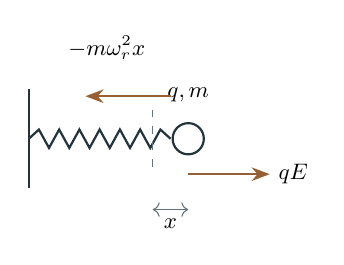
\begin{tikzpicture}[scale=.9,transform shape]
\draw[object] (0.00000,-0.70000)--(0.00000,0.70000);\draw[object] plot coordinates {(0.00000,0.00000) (0.14286,0.13000) (0.28571,-0.13000) (0.42857,0.13000) (0.57143,-0.13000) (0.71429,0.13000) (0.85714,-0.13000) (1.00000,0.13000) (1.14286,-0.13000) (1.28571,0.13000) (1.42857,-0.13000) (1.57143,0.13000) (1.71429,-0.13000) (1.85714,0.13000) (2.00000,0.00000)};\draw[object] (2.25000,0.00000) circle(0.22000);\node[above] at (2.25000,0.40000) {$q,m$};\draw[force] (2.25000,-0.50000)--(3.40000,-0.50000);\node[right] at (3.40000,-0.50000) {$qE$};\draw[force] (2.00000,0.60000)--(0.80000,0.60000);\node[above] at (1.10000,1.00000) {$-m\omega_r^2x$};\draw[<->,thin,color=muted] (1.75000,-1.00000)--(2.25000,-1.00000);\node[below] at (2.00000,-1.00000) {$x$};\draw[guide] (1.75000,-0.40000)--(1.75000,0.40000);
\end{tikzpicture}
\figcaption{图光5.2\quad 束缚振子的外力、回复力与位移。}
\end{minipage}\end{center}

\workarea

\clearpage

\pdfbookmark[2]{第 3 题 双共振色散与质量比}{q3}

\section*{第 3 题\quad 双共振色散与质量比}\label{q:3}

氟化钙在$0.3$至$10\,\mu\mathrm m$波段有经验关系
\[
n^2=6.09+\frac{6.12\times10^{-15}}{\lambda_0^2-8.88\times10^{-15}}
+\frac{5.10\times10^{-9}}{\lambda_0^2-1.26\times10^{-9}},
\]
式中长度均以m计。求两个有效共振吸收波长。再在两类振子数相等、有效电荷大小相等的近似下，以第一类质量为$m_e$、第二类为Ca与F相对振动的约化质量，估算$m_{\mathrm H}/m_e$。取Ca、F相对原子质量40、19，并检查经验式常数项与双振子模型的关系。

\begin{center}\begin{minipage}{.98\linewidth}\centering
\begin{tikzpicture}[scale=.9,transform shape]
\draw[object] (0.80000,0.00000) circle(0.36000);\draw[object] (4.00000,0.00000) circle(0.25000);\draw[object] plot coordinates {(1.16000,0.00000) (1.34500,0.13000) (1.53000,-0.13000) (1.71500,0.13000) (1.90000,-0.13000) (2.08500,0.13000) (2.27000,-0.13000) (2.45500,0.13000) (2.64000,-0.13000) (2.82500,0.13000) (3.01000,-0.13000) (3.19500,0.13000) (3.38000,-0.13000) (3.56500,0.13000) (3.75000,0.00000)};\node[above] at (0.80000,0.50000) {Ca};\node[above] at (4.00000,0.50000) {F};\draw[force] (0.80000,-0.50000)--(0.20000,-0.50000);\draw[force] (4.00000,-0.50000)--(4.90000,-0.50000);\draw[<->,thin,color=muted] (0.80000,-1.10000)--(4.00000,-1.10000);\node[below] at (2.40000,-1.10000) {相对位移 $x_{\rm Ca}-x_{\rm F}$};\node[above] at (2.40000,1.10000) {$\mu=m_{\rm Ca}m_{\rm F}/(m_{\rm Ca}+m_{\rm F})$};
\end{tikzpicture}
\figcaption{图光5.3\quad Ca与F的相对运动使用约化质量。}
\end{minipage}\end{center}

\workarea

\clearpage

\pdfbookmark[2]{第 4 题 X射线色散及速度乘积}{q4}

\section*{第 4 题\quad X射线色散及速度乘积}\label{q:4}

在X射线频率远高于电子束缚共振频率、损耗可忽略的范围内，证明金属折射率满足$n^2=1-K\lambda_0^2$。对铜取原子序数29、相对原子质量63、密度$8.0\times10^3\,\mathrm{kg/m^3}$，估算$K$；再证明该模型内相速与群速的乘积为$c^2$。

\begin{center}\begin{minipage}{.98\linewidth}\centering
\begin{tikzpicture}[scale=.9,transform shape]
\draw[axis] (0.00000,0.00000)--(6.80000,0.00000);\draw[axis] (0.00000,-0.15000)--(0.00000,2.30000);\node[below right] at (6.80000,0.00000) {$\omega/\omega_p$};\node[above right] at (0.00000,2.30000) {$n^2$};\draw[traj] plot coordinates {(1.00000,0.00000) (1.03741,0.14164) (1.07482,0.26876) (1.11223,0.38326) (1.14964,0.48677) (1.18705,0.58064) (1.22446,0.66605) (1.26187,0.74397) (1.29928,0.81526) (1.33669,0.88064) (1.37410,0.94076) (1.41151,0.99617) (1.44892,1.04733) (1.48633,1.09469) (1.52374,1.13859) (1.56115,1.17938) (1.59856,1.21734) (1.63597,1.25273) (1.67338,1.28577) (1.71079,1.31666) (1.74820,1.34559) (1.78561,1.37273) (1.82302,1.39821) (1.86043,1.42217) (1.89784,1.44472) (1.93525,1.46598) (1.97266,1.48605) (2.01007,1.50500) (2.04748,1.52292) (2.08489,1.53989) (2.12230,1.55597) (2.15971,1.57122) (2.19712,1.58569) (2.23453,1.59945) (2.27194,1.61253) (2.30935,1.62498) (2.34676,1.63685) (2.38417,1.64815) (2.42158,1.65894) (2.45899,1.66924) (2.49640,1.67908) (2.53381,1.68848) (2.57122,1.69748) (2.60863,1.70610) (2.64604,1.71435) (2.68345,1.72226) (2.72086,1.72984) (2.75827,1.73712) (2.79568,1.74411) (2.83309,1.75082) (2.87050,1.75728) (2.90791,1.76348) (2.94532,1.76945) (2.98273,1.77520) (3.02014,1.78073) (3.05755,1.78607) (3.09496,1.79121) (3.13237,1.79616) (3.16978,1.80095) (3.20719,1.80556) (3.24460,1.81002) (3.28201,1.81433) (3.31942,1.81849) (3.35683,1.82251) (3.39424,1.82640) (3.43165,1.83017) (3.46906,1.83381) (3.50647,1.83734) (3.54388,1.84075) (3.58129,1.84406) (3.61871,1.84727) (3.65612,1.85038) (3.69353,1.85340) (3.73094,1.85632) (3.76835,1.85916) (3.80576,1.86191) (3.84317,1.86459) (3.88058,1.86719) (3.91799,1.86971) (3.95540,1.87216) (3.99281,1.87455) (4.03022,1.87687) (4.06763,1.87912) (4.10504,1.88131) (4.14245,1.88345) (4.17986,1.88553) (4.21727,1.88755) (4.25468,1.88952) (4.29209,1.89143) (4.32950,1.89330) (4.36691,1.89512) (4.40432,1.89690) (4.44173,1.89863) (4.47914,1.90031) (4.51655,1.90196) (4.55396,1.90356) (4.59137,1.90513) (4.62878,1.90665) (4.66619,1.90814) (4.70360,1.90960) (4.74101,1.91102) (4.77842,1.91241) (4.81583,1.91376) (4.85324,1.91509) (4.89065,1.91638) (4.92806,1.91765) (4.96547,1.91888) (5.00288,1.92009) (5.04029,1.92127) (5.07770,1.92243) (5.11511,1.92356) (5.15252,1.92467) (5.18993,1.92575) (5.22734,1.92681) (5.26475,1.92784) (5.30216,1.92886) (5.33957,1.92985) (5.37698,1.93082) (5.41439,1.93178) (5.45180,1.93271) (5.48921,1.93362) (5.52662,1.93452) (5.56403,1.93540) (5.60144,1.93626) (5.63885,1.93710) (5.67626,1.93793) (5.71367,1.93874) (5.75108,1.93953) (5.78849,1.94031) (5.82590,1.94107) (5.86331,1.94182) (5.90072,1.94256) (5.93813,1.94328) (5.97554,1.94399) (6.01295,1.94468) (6.05036,1.94537) (6.08777,1.94603) (6.12518,1.94669) (6.16259,1.94734) (6.20000,1.94797)};\draw[guide] (0.00000,2.00000)--(6.20000,2.00000);\node[left] at (0.00000,2.00000) {1};\node[below] at (1.00000,0.00000) {1};
\end{tikzpicture}
\figcaption{图光5.4\quad 高频传播区的折射率平方从零趋近1。}
\end{minipage}\end{center}

\workarea

\clearpage

\pdfbookmark[2]{第 5 题 金属自由电子响应与反射}{q5}

\section*{第 5 题\quad 金属自由电子响应与反射}\label{q:5}

假设影响金属光学性质的是数密度为$N$的自由价电子，忽略磁响应及束缚电子背景。导出弱阻尼下的色散关系，求真空光正入射半无限金属时能量反射率随真空波长的关系。区分传播区、倏逝区和真正的吸收，并说明有限阻尼怎样改变结果。

\begin{center}\begin{minipage}{.98\linewidth}\centering
\begin{tikzpicture}[scale=.9,transform shape]
\draw[object] (3.00000,-1.30000)--(3.00000,1.50000);\node[above] at (1.00000,1.20000) {真空};\node[above] at (5.00000,1.20000) {金属 $z>0$};\draw[motion] (0.00000,0.50000)--(3.00000,0.50000);\node[above right] at (0.30000,0.50000) {入射};\draw[force] (3.00000,-0.10000)--(0.20000,-0.10000);\node[below right] at (0.40000,-0.10000) {反射};\draw[axis] (3.00000,0.00000)--(6.80000,0.00000);\node[below right] at (6.80000,0.00000) {$z$};\draw[traj] plot coordinates {(3.00000,0.80000) (3.03434,0.77698) (3.06869,0.75463) (3.10303,0.73292) (3.13737,0.71183) (3.17172,0.69135) (3.20606,0.67146) (3.24040,0.65215) (3.27475,0.63338) (3.30909,0.61516) (3.34343,0.59746) (3.37778,0.58027) (3.41212,0.56358) (3.44646,0.54737) (3.48081,0.53162) (3.51515,0.51632) (3.54949,0.50147) (3.58384,0.48704) (3.61818,0.47303) (3.65253,0.45942) (3.68687,0.44620) (3.72121,0.43337) (3.75556,0.42090) (3.78990,0.40879) (3.82424,0.39703) (3.85859,0.38561) (3.89293,0.37451) (3.92727,0.36374) (3.96162,0.35327) (3.99596,0.34311) (4.03030,0.33324) (4.06465,0.32365) (4.09899,0.31434) (4.13333,0.30529) (4.16768,0.29651) (4.20202,0.28798) (4.23636,0.27970) (4.27071,0.27165) (4.30505,0.26383) (4.33939,0.25624) (4.37374,0.24887) (4.40808,0.24171) (4.44242,0.23476) (4.47677,0.22800) (4.51111,0.22144) (4.54545,0.21507) (4.57980,0.20888) (4.61414,0.20288) (4.64848,0.19704) (4.68283,0.19137) (4.71717,0.18586) (4.75152,0.18052) (4.78586,0.17532) (4.82020,0.17028) (4.85455,0.16538) (4.88889,0.16062) (4.92323,0.15600) (4.95758,0.15151) (4.99192,0.14715) (5.02626,0.14292) (5.06061,0.13881) (5.09495,0.13482) (5.12929,0.13094) (5.16364,0.12717) (5.19798,0.12351) (5.23232,0.11996) (5.26667,0.11651) (5.30101,0.11315) (5.33535,0.10990) (5.36970,0.10674) (5.40404,0.10367) (5.43838,0.10068) (5.47273,0.09779) (5.50707,0.09497) (5.54141,0.09224) (5.57576,0.08959) (5.61010,0.08701) (5.64444,0.08451) (5.67879,0.08208) (5.71313,0.07971) (5.74747,0.07742) (5.78182,0.07519) (5.81616,0.07303) (5.85051,0.07093) (5.88485,0.06889) (5.91919,0.06691) (5.95354,0.06498) (5.98788,0.06311) (6.02222,0.06130) (6.05657,0.05953) (6.09091,0.05782) (6.12525,0.05616) (6.15960,0.05454) (6.19394,0.05297) (6.22828,0.05145) (6.26263,0.04997) (6.29697,0.04853) (6.33131,0.04713) (6.36566,0.04578) (6.40000,0.04446)};\node[above right] at (5.20000,0.50000) {倏逝包络};
\end{tikzpicture}
\figcaption{图光5.5\quad 半无限金属表面及倏逝区的空间衰减。}
\end{minipage}\end{center}

\workarea

\clearpage

\pdfbookmark[2]{第 6 题 电离层的反射与布儒斯特角}{q6}

\section*{第 6 题\quad 电离层的反射与布儒斯特角}\label{q:6}

将电离层看作均匀、无碰撞、无外磁场的冷等离子体，电子数密度为$N$，重离子响应忽略。它与非电离大气之间有平面突变界面，大气折射率取1。（1）当$\nu=2\nu_p$或$\nu\ll\nu_p$时，求从大气正入射的能量反射率，其中$\nu_p$为等离子体频率。（2）在允许传播的情形，若反射光只含垂直于入射面的振动，入射角应是多少？明确给出$\nu=2\nu_p$的结果。

\begin{center}\begin{minipage}{.98\linewidth}\centering
\begin{tikzpicture}[scale=.9,transform shape]
\draw[object] (-3.00000,0.00000)--(3.00000,0.00000);\node[left] at (-0.70000,1.40000) {大气 $n_1=1$};\node[below] at (0.00000,-2.80000) {等离子体 $\varepsilon=1-\nu_p^2/\nu^2$};\draw[motion] (-0.20000,2.00000)--(-0.20000,0.00000);
\draw[motion] (-0.20000,0.00000)--(-0.20000,-2.00000);\draw[force] (0.20000,0.00000)--(0.20000,2.00000);\node[right] at (0.80000,1.00000) {反射 $R$};
\end{tikzpicture}
\figcaption{图光5.6\quad 正入射能量分配先按频率区间判断。}
\end{minipage}\end{center}

\workarea

\clearpage

\pdfbookmark[2]{第 7 题 麦克斯韦方程的纵向模式}{q7}

\section*{第 7 题\quad 麦克斯韦方程的纵向模式}\label{q:7}

对均匀、各向同性、非磁性的介质，讨论无外加自由电荷和电流时，麦克斯韦方程存在非零频率平面纵向电场模式的条件。把条件用于无碰撞冷等离子体，求其频率、磁场及群速，说明它与横向电磁波的区别。允许介质内部的感应电荷和电流。

\begin{center}\begin{minipage}{.98\linewidth}\centering
\begin{tikzpicture}[scale=.9,transform shape]
\draw[axis] (0.00000,0.00000)--(8.30000,0.00000);\draw[axis] (0.00000,-0.15000)--(0.00000,2.00000);\node[below right] at (8.30000,0.00000) {$z$};\node[above right] at (0.00000,2.00000) {$\xi,E$};\draw[traj] plot coordinates {(0.00000,0.00000) (0.04020,0.05048) (0.08040,0.10077) (0.12060,0.15065) (0.16080,0.19993) (0.20101,0.24841) (0.24121,0.29591) (0.28141,0.34222) (0.32161,0.38717) (0.36181,0.43058) (0.40201,0.47227) (0.44221,0.51208) (0.48241,0.54984) (0.52261,0.58542) (0.56281,0.61866) (0.60302,0.64943) (0.64322,0.67762) (0.68342,0.70310) (0.72362,0.72579) (0.76382,0.74557) (0.80402,0.76239) (0.84422,0.77617) (0.88442,0.78685) (0.92462,0.79440) (0.96482,0.79878) (1.00503,0.79998) (1.04523,0.79798) (1.08543,0.79281) (1.12563,0.78447) (1.16583,0.77301) (1.20603,0.75847) (1.24623,0.74090) (1.28643,0.72038) (1.32663,0.69699) (1.36683,0.67082) (1.40704,0.64198) (1.44724,0.61057) (1.48744,0.57674) (1.52764,0.54060) (1.56784,0.50231) (1.60804,0.46202) (1.64824,0.41988) (1.68844,0.37607) (1.72864,0.33076) (1.76884,0.28414) (1.80905,0.23638) (1.84925,0.18768) (1.88945,0.13823) (1.92965,0.08823) (1.96985,0.03787) (2.01005,-0.01263) (2.05025,-0.06308) (2.09045,-0.11328) (2.13065,-0.16303) (2.17085,-0.21213) (2.21106,-0.26039) (2.25126,-0.30760) (2.29146,-0.35359) (2.33166,-0.39818) (2.37186,-0.44117) (2.41206,-0.48240) (2.45226,-0.52172) (2.49246,-0.55895) (2.53266,-0.59395) (2.57286,-0.62659) (2.61307,-0.65673) (2.65327,-0.68425) (2.69347,-0.70904) (2.73367,-0.73101) (2.77387,-0.75006) (2.81407,-0.76612) (2.85427,-0.77913) (2.89447,-0.78903) (2.93467,-0.79579) (2.97487,-0.79938) (3.01508,-0.79978) (3.05528,-0.79699) (3.09548,-0.79102) (3.13568,-0.78190) (3.17588,-0.76966) (3.21608,-0.75436) (3.25628,-0.73605) (3.29648,-0.71480) (3.33668,-0.69071) (3.37688,-0.66386) (3.41709,-0.63436) (3.45729,-0.60234) (3.49749,-0.56791) (3.53769,-0.53122) (3.57789,-0.49242) (3.61809,-0.45165) (3.65829,-0.40908) (3.69849,-0.36488) (3.73869,-0.31922) (3.77889,-0.27230) (3.81910,-0.22428) (3.85930,-0.17538) (3.89950,-0.12577) (3.93970,-0.07566) (3.97990,-0.02525) (4.02010,0.02525) (4.06030,0.07566) (4.10050,0.12577) (4.14070,0.17538) (4.18090,0.22428) (4.22111,0.27230) (4.26131,0.31922) (4.30151,0.36488) (4.34171,0.40908) (4.38191,0.45165) (4.42211,0.49242) (4.46231,0.53122) (4.50251,0.56791) (4.54271,0.60234) (4.58291,0.63436) (4.62312,0.66386) (4.66332,0.69071) (4.70352,0.71480) (4.74372,0.73605) (4.78392,0.75436) (4.82412,0.76966) (4.86432,0.78190) (4.90452,0.79102) (4.94472,0.79699) (4.98492,0.79978) (5.02513,0.79938) (5.06533,0.79579) (5.10553,0.78903) (5.14573,0.77913) (5.18593,0.76612) (5.22613,0.75006) (5.26633,0.73101) (5.30653,0.70904) (5.34673,0.68425) (5.38693,0.65673) (5.42714,0.62659) (5.46734,0.59395) (5.50754,0.55895) (5.54774,0.52172) (5.58794,0.48240) (5.62814,0.44117) (5.66834,0.39818) (5.70854,0.35359) (5.74874,0.30760) (5.78894,0.26039) (5.82915,0.21213) (5.86935,0.16303) (5.90955,0.11328) (5.94975,0.06308) (5.98995,0.01263) (6.03015,-0.03787) (6.07035,-0.08823) (6.11055,-0.13823) (6.15075,-0.18768) (6.19095,-0.23638) (6.23116,-0.28414) (6.27136,-0.33076) (6.31156,-0.37607) (6.35176,-0.41988) (6.39196,-0.46202) (6.43216,-0.50231) (6.47236,-0.54060) (6.51256,-0.57674) (6.55276,-0.61057) (6.59296,-0.64198) (6.63317,-0.67082) (6.67337,-0.69699) (6.71357,-0.72038) (6.75377,-0.74090) (6.79397,-0.75847) (6.83417,-0.77301) (6.87437,-0.78447) (6.91457,-0.79281) (6.95477,-0.79798) (6.99497,-0.79998) (7.03518,-0.79878) (7.07538,-0.79440) (7.11558,-0.78685) (7.15578,-0.77617) (7.19598,-0.76239) (7.23618,-0.74557) (7.27638,-0.72579) (7.31658,-0.70310) (7.35678,-0.67762) (7.39698,-0.64943) (7.43719,-0.61866) (7.47739,-0.58542) (7.51759,-0.54984) (7.55779,-0.51208) (7.59799,-0.47227) (7.63819,-0.43058) (7.67839,-0.38717) (7.71859,-0.34222) (7.75879,-0.29591) (7.79899,-0.24841) (7.83920,-0.19993) (7.87940,-0.15065) (7.91960,-0.10077) (7.95980,-0.05048) (8.00000,-0.00000)};\node[above] at (2.00000,1.40000) {电子层位移 $\xi$，$E=eN\xi/\varepsilon_0$};\draw[thin,color=accent] (0.40896,-0.75000)--(0.40896,-1.15000);\draw[thin,color=accent] (1.05992,-0.75000)--(1.05992,-1.15000);\draw[thin,color=accent] (1.56036,-0.75000)--(1.56036,-1.15000);\draw[thin,color=accent] (1.92857,-0.75000)--(1.92857,-1.15000);\draw[thin,color=accent] (2.26890,-0.75000)--(2.26890,-1.15000);\draw[thin,color=accent] (2.70382,-0.75000)--(2.70382,-1.15000);\draw[thin,color=accent] (3.29428,-0.75000)--(3.29428,-1.15000);\draw[thin,color=accent] (4.00000,-0.75000)--(4.00000,-1.15000);\draw[thin,color=accent] (4.70572,-0.75000)--(4.70572,-1.15000);\draw[thin,color=accent] (5.29618,-0.75000)--(5.29618,-1.15000);\draw[thin,color=accent] (5.73110,-0.75000)--(5.73110,-1.15000);\draw[thin,color=accent] (6.07143,-0.75000)--(6.07143,-1.15000);\draw[thin,color=accent] (6.43964,-0.75000)--(6.43964,-1.15000);\draw[thin,color=accent] (6.94008,-0.75000)--(6.94008,-1.15000);\draw[thin,color=accent] (7.59104,-0.75000)--(7.59104,-1.15000);\node[below] at (2.00000,-1.50000) {压缩区};\node[below] at (4.00000,-1.50000) {稀疏区};\node[below] at (7.00000,-1.50000) {$\boldsymbol H=0$};
\end{tikzpicture}
\figcaption{图光5.7\quad 纵向位移、回复电场与电子层密度变化。}
\end{minipage}\end{center}

\workarea

\clearpage

\pdfbookmark[2]{第 8 题 均匀介质与涨落散射}{q8}

\section*{第 8 题\quad 均匀介质与涨落散射}\label{q:8}

根据经典电磁理论，说明无限均匀、无密度涨落的介质为何没有偏离前向的体散射；再把介质分为许多尺寸远小于波长的微元，设微元响应振幅相对均值的涨落为$\Delta A_j$，证明在互不相关的零均值涨落条件下，平均散射强度与$\langle|\Delta A|^2\rangle$成正比。说明样品的有限尺寸及空间相关会怎样改变论证。

\begin{center}\begin{minipage}{.98\linewidth}\centering
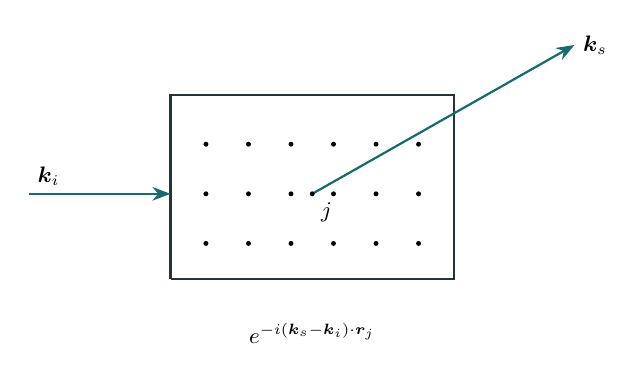
\begin{tikzpicture}[scale=.9,transform shape]
\draw[object] (0.00000,-1.00000)--(4.00000,-1.00000)--(4.00000,1.60000)--(0.00000,1.60000)--(0.00000,-1.00000);\fill (0.50000,-0.50000) circle(.035);\fill (0.50000,0.20000) circle(.035);\fill (0.50000,0.90000) circle(.035);\fill (1.10000,-0.50000) circle(.035);\fill (1.10000,0.20000) circle(.035);\fill (1.10000,0.90000) circle(.035);\fill (1.70000,-0.50000) circle(.035);\fill (1.70000,0.20000) circle(.035);\fill (1.70000,0.90000) circle(.035);\fill (2.30000,-0.50000) circle(.035);\fill (2.30000,0.20000) circle(.035);\fill (2.30000,0.90000) circle(.035);\fill (2.90000,-0.50000) circle(.035);\fill (2.90000,0.20000) circle(.035);\fill (2.90000,0.90000) circle(.035);\fill (3.50000,-0.50000) circle(.035);\fill (3.50000,0.20000) circle(.035);\fill (3.50000,0.90000) circle(.035);\draw[motion] (-2.00000,0.20000)--(0.00000,0.20000);\node[above right] at (-2.00000,0.20000) {$\boldsymbol k_i$};\draw[motion] (2.00000,0.20000)--(5.70000,2.30000);\node[right] at (5.70000,2.30000) {$\boldsymbol k_s$};\fill (2.00000,0.20000) circle(.035);\node[below right] at (2.00000,0.20000) {$j$};\node[below] at (2.00000,-1.50000) {$e^{-i(\boldsymbol k_s-\boldsymbol k_i)\cdot\boldsymbol r_j}$};
\end{tikzpicture}
\figcaption{图光5.8\quad 每个微元的相位由入射与出射方向共同决定。}
\end{minipage}\end{center}

\workarea

\clearpage

\pdfbookmark[2]{第 9 题 密度涨落的瑞利散射}{q9}

\section*{第 9 题\quad 密度涨落的瑞利散射}\label{q:9}

自然光沿$z$轴入射弱色散、光学稀薄介质。相对介电常数依赖密度$\rho$，在考察波段中$\partial\varepsilon_r/\partial\rho$可视为常量，温度对它的直接影响忽略。以远小于波长的微元作为电偶极子，由经典偶极辐射证明：短程、各向同性密度涨落造成的远场散射在角度$\theta$处满足
\[
I_\theta\propto\frac{1+\cos^2\theta}{\lambda_0^4}.
\]
给出振幅叠加、统计平均及偏振因子的推导，并说明比例式的适用条件。可用偶极远场幅度$E_s=\omega^2p\sin\alpha/(4\pi\varepsilon_0c^2r)$。

\begin{center}\begin{minipage}{.98\linewidth}\centering
\begin{tikzpicture}[scale=.9,transform shape]
\draw[axis] (-3.00000,0.00000)--(0.00000,0.00000);
\draw[axis] (0.00000,0.00000)--(3.20000,0.00000);\node[below right] at (3.20000,0.00000) {$z,\boldsymbol k_i$};\draw[axis] (0.00000,0.00000)--(0.00000,2.40000);\node[above right] at (0.00000,2.40000) {$x$};\draw[axis] (0.00000,0.00000)--(-1.30000,-1.00000);\node[below left] at (-1.30000,-1.00000) {$y$};\fill (0.00000,0.00000) circle(.035);\node[below right] at (0.00000,0.00000) {$O$};\draw[force] (0.00000,0.00000)--(2.80000,2.10000);\node[above right] at (2.80000,2.10000) {观察方向 $\boldsymbol s$};\node[above] at (1.00000,0.28000) {$\theta$};\node[above right] at (-3.00000,0.30000) {自然光};\node[below] at (1.00000,-2.00000) {散射面为 $xz$；$s$偏振垂直该面};
\end{tikzpicture}
\figcaption{图光5.9\quad 自然光两横向分量与观察方向的几何关系。}
\end{minipage}\end{center}

\workarea

\clearpage

\pdfbookmark[2]{第 10 题 射电脉冲啁啾与电子密度}{q10}

\section*{第 10 题\quad 射电脉冲啁啾与电子密度}\label{q:10}

距离地球$L$的空间射电源，在同一时刻发出宽频带短脉冲。假设传播路径是均匀、无磁场、无碰撞的完全电离冷等离子体，传播频率高于等离子体截止频率。到达信号的角频率随接收时刻变化，局部斜率$\dd\omega/\dd t$已测得。由$L$、该时刻角频率$\omega$和斜率，导出电子平均数密度$N$的确定式；同时给出高频近似，并说明反演需要的发射条件。

\begin{center}\begin{minipage}{.98\linewidth}\centering
\begin{tikzpicture}[scale=.9,transform shape]
\fill (0.00000,0.00000) circle(.035);\node[left] at (0.00000,0.00000) {射电源};\draw[object] (7.00000,-1.50000)--(7.00000,1.80000);\node[above] at (7.00000,1.80000) {地球};\draw[motion] (0.00000,0.00000)--(2.00000,1.00000);
\draw[motion] (2.00000,1.00000)--(6.50000,1.00000);\node[above] at (3.80000,1.12000) {高频先到};\draw[motion] (0.00000,0.00000)--(2.00000,0.00000);
\draw[motion] (2.00000,0.00000)--(6.50000,0.00000);\node[above] at (3.80000,0.12000) {中心频率};\draw[motion] (0.00000,0.00000)--(2.00000,-1.00000);
\draw[motion] (2.00000,-1.00000)--(6.50000,-1.00000);\node[above] at (3.80000,-0.88000) {低频后到};\draw[<->,thin,color=muted] (0.00000,-2.00000)--(7.00000,-2.00000);\node[below] at (3.50000,-2.00000) {传播长度 $L$};\node[above] at (1.00000,2.00000) {共同发射时刻 $t_e$};
\end{tikzpicture}
\figcaption{图光5.10\quad 频率分量同时发射，群延迟使接收时间分开。}
\end{minipage}\end{center}

\workarea

\clearpage

\pdfbookmark[2]{第 11 题 吸收系数测量与表面反射}{q11}

\section*{第 11 题\quad 吸收系数测量与表面反射}\label{q:11}

强度$I_0$的单色光从空气垂直入射厚度$l$的有色玻璃，玻璃折射率$n=1.5$，强度吸收系数为$\alpha$。（1）忽略多重反射，求透射强度与入射强度之比。（2）忽略表面反射损失会产生多大的相对误差？明确误差以哪个量为分母，并给小反射率的一阶结果。（3）设计消除表面反射影响的吸收系数测量方法，说明需要保持哪些条件。

\begin{center}\begin{minipage}{.98\linewidth}\centering
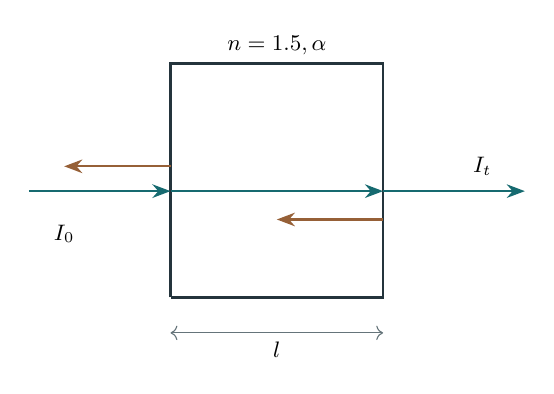
\begin{tikzpicture}[scale=.9,transform shape]
\draw[object] (2.00000,-1.50000)--(2.00000,1.80000)--(5.00000,1.80000)--(5.00000,-1.50000)--(2.00000,-1.50000);\node[above] at (3.50000,1.80000) {$n=1.5,\alpha$};\draw[motion] (0.00000,0.00000)--(2.00000,0.00000);
\draw[motion] (2.00000,0.00000)--(5.00000,0.00000);
\draw[motion] (5.00000,0.00000)--(7.00000,0.00000);\node[below] at (0.50000,-0.35000) {$I_0$};\node[above] at (6.40000,0.10000) {$I_t$};\draw[force] (2.00000,0.35000)--(0.50000,0.35000);\draw[force] (5.00000,-0.40000)--(3.50000,-0.40000);\draw[<->,thin,color=muted] (2.00000,-2.00000)--(5.00000,-2.00000);\node[below] at (3.50000,-2.00000) {$l$};
\end{tikzpicture}
\figcaption{图光5.11\quad 光经历入口反射、体吸收与出口反射。}
\end{minipage}\end{center}

\workarea

\end{document}
